\documentclass[a4paper,oneside,12pt]{extreport}

\usepackage{mmap}
\usepackage[T2A]{fontenc}
\usepackage[utf8]{inputenc}
\usepackage[english,russian]{babel}

\usepackage[left=30mm, right=15mm, top=20mm, bottom=20mm]{geometry}

\setlength{\parindent}{1.25cm} % Абзацный отступ

\usepackage{setspace}
\onehalfspacing % Полуторный интервал

\frenchspacing % Равномерные пробелы
\usepackage{indentfirst} % Красная строка

\usepackage{microtype}
\sloppy

\usepackage{titlesec}
\titlespacing*{\chapter}{0pt}{-30pt}{8pt}
\titlespacing*{\section}{\parindent}{*4}{*4}
\titlespacing*{\subsection}{\parindent}{*4}{*4}
\titleformat{\chapter}{\LARGE\bfseries}{\thechapter}{20pt}{\LARGE\bfseries}
\titleformat{\section}{\Large\bfseries}{\thesection}{40pt}{\Large\bfseries}

\usepackage{graphicx}
\usepackage{caption}

\usepackage[unicode,pdftex]{hyperref}
\hypersetup{hidelinks}

\usepackage{amsmath}

%% title begin
\usepackage{wrapfig}

\makeatletter
	\def\vhrulefill#1{\leavevmode\leaders\hrule\@height#1\hfill \kern\z@}
\makeatother
%% title end

%% begin code
\usepackage{listings}
\usepackage{xcolor}

\lstset{
	basicstyle=\footnotesize\ttfamily,
	breakatwhitespace=true,
	breaklines=true,
	commentstyle=\color{gray},
	frame=single,
	keywordstyle=\color{blue},
	stringstyle=\color{red},
	tabsize=8
}

\newcommand{\code}[1]{\texttt{#1}}
%% end code


\begin{document}

\begin{titlepage}
	{\large % 14pt instead of 12pt
	\onehalfspacing
	\centering

	\begin{wrapfigure}[7]{l}{0.14\linewidth}
		\vspace{3mm}
		\hspace{-10mm}
		
\includegraphics[width=0.93\linewidth]{inc/img/bmstu-logo}
	\end{wrapfigure}
	{\singlespacing \footnotesize \bfseries Министерство науки и высшего образования Российской Федерации\\Федеральное государственное бюджетное образовательное учреждение\\высшего образования\\<<Московский государственный технический университет\\имени Н.~Э.~Баумана\\ (национальный исследовательский университет)>>\\(МГТУ им. Н.~Э.~Баумана)\\}

	\vspace{-2.2mm}
	\vhrulefill{0.9mm}\\
	\vspace{-7.5mm}
	\vhrulefill{0.2mm}\\
	\vspace{2mm}

	{\doublespacing \small \raggedright ФАКУЛЬТЕТ \hspace{37mm} «Информатика и системы управления»\\
	КАФЕДРА \hspace{17mm} «Программное обеспечение ЭВМ и информационные технологии»\\}

	\vspace{30mm}

	\textbf{ОТЧЁТ}\\
	По лабораторной работе № 2\\
	По курсу: «Моделирование»\\
	Тема: «Распределение случайных величин»\\
	Вариант: 6 $\equiv$ 2 (mod 4)\\

	\vspace{40mm}

	\begin{flushleft}
		\begin{tabular}{lr}
			\textbf{Студент:}        & Керимов~А.~Ш. \\
			\textbf{Группа:}         & ИУ7-74Б       \\
			\textbf{Оценка (баллы):} & \hrulefill    \\
			\textbf{Преподаватель:}  & Рудаков~И.~В. \\
		\end{tabular}
	\end{flushleft}

	\vfill

	Москва\\
	\the\year\\}
\end{titlepage}

\setcounter{page}{2}


\tableofcontents

\chapter{Формализация}

\section{Задание}

Смоделировать марковский процесс, имеющий не более 10 состояний, для каждого из которых рассчитать предельную вероятность и время стабилизации.

\section{Теория}

Случайный процесс называется марковским, если он обладает следующим свойством: для каждого момента времени $t_0$ вероятность любого состояния системы в будущем зависит только от её состояния в настоящем (при $t = t_0$) и не зависит от того, когда и каким образом система пришла в это состояние, т. е. не зависит от того, как процесс развивался в прошлом.

Пусть в системе $n$ состояний $\{S_1, \ldots, S_n\}$.
Функционирование этой системы задаётся размеченным графом: узлы — состояния, дуги — интенсивности переходов системы $\lambda_{ij}$ из состояния $S_i$ в состояние $S_j$.
Матрица интенсивностей:
\begin{equation}
	\Lambda = \begin{pmatrix}
		&0 &\lambda_{12} &\lambda_{13} &\ldots &\lambda_{1n} \\
		&\lambda_{21} &0 &\lambda_{23} &\ldots &\lambda_{2n} \\
		&\lambda_{31} &\lambda_{32} &0 &\ldots &\lambda_{3n} \\
		&\vdots &\vdots &\vdots &\ddots &\vdots \\
		&\lambda_{n1} &\lambda_{n2} &\lambda_{n3} &\ldots &0 \\
	\end{pmatrix}
\end{equation}

Вероятность нахождения системы в состоянии $S_i$ в момент времени $t$ обозначается $p_i(t)$ и описывается уравнением Колмогорова:
\begin{equation}
	\label{eqn:kolmogorov}
	\frac{\mathrm dp_i(t)}{\mathrm dt} = \sum_{j = 1}^{n} \lambda_{ji} p_j(t) - p_i(t) \sum_{j = 1}^{n} \lambda_{ij}.
\end{equation}

Предельная вероятность состояния $S_i$: $\displaystyle \lim_{t \to \infty} p_i(t)$, она характеризует установившийся режим работы системы.
Для предельных вероятностей справедливо уравнение нормировки:
\begin{equation}
	\label{eqn:norm}
	\sum_{i = 1}^{n} \left(\lim_{t \to \infty} p_i(t)\right) = 1
\end{equation}

Для нахождения предельных вероятностей недостаточно приравнять к нулю производные в уравнениях \eqref{eqn:kolmogorov}, т. к. в системе независимых уравнений на единицу меньше $n$.
Поэтому необходимо заменить одно любое уравнение на уравнение нормировки \eqref{eqn:norm}.

Для нахождения времени стабилизации $t$ системы необходимо находить вероятности состояний с шагом $\Delta t$ до условия: $\displaystyle \Bigg(\abs{p_i(t + \Delta t) - p_i(t)} < \varepsilon\Bigg) \; \& \; \Bigg(\abs{p_i(t) - \lim_{t \to \infty}p_i(t)} < \varepsilon\Bigg)$.

\chapter{Результат работы}

В столбце $t1$ выведено время стабилизации для следующих вероятностей состояний системы в начальный момент времени: $p_1(0) = 1, p_i(0) = 0, i = \overline{2, n}$.
В столбце $t2$ — для $p_j(0) = 1 / n, j = \overline{1, n}$.

\begin{figure}[H]
	\centering
	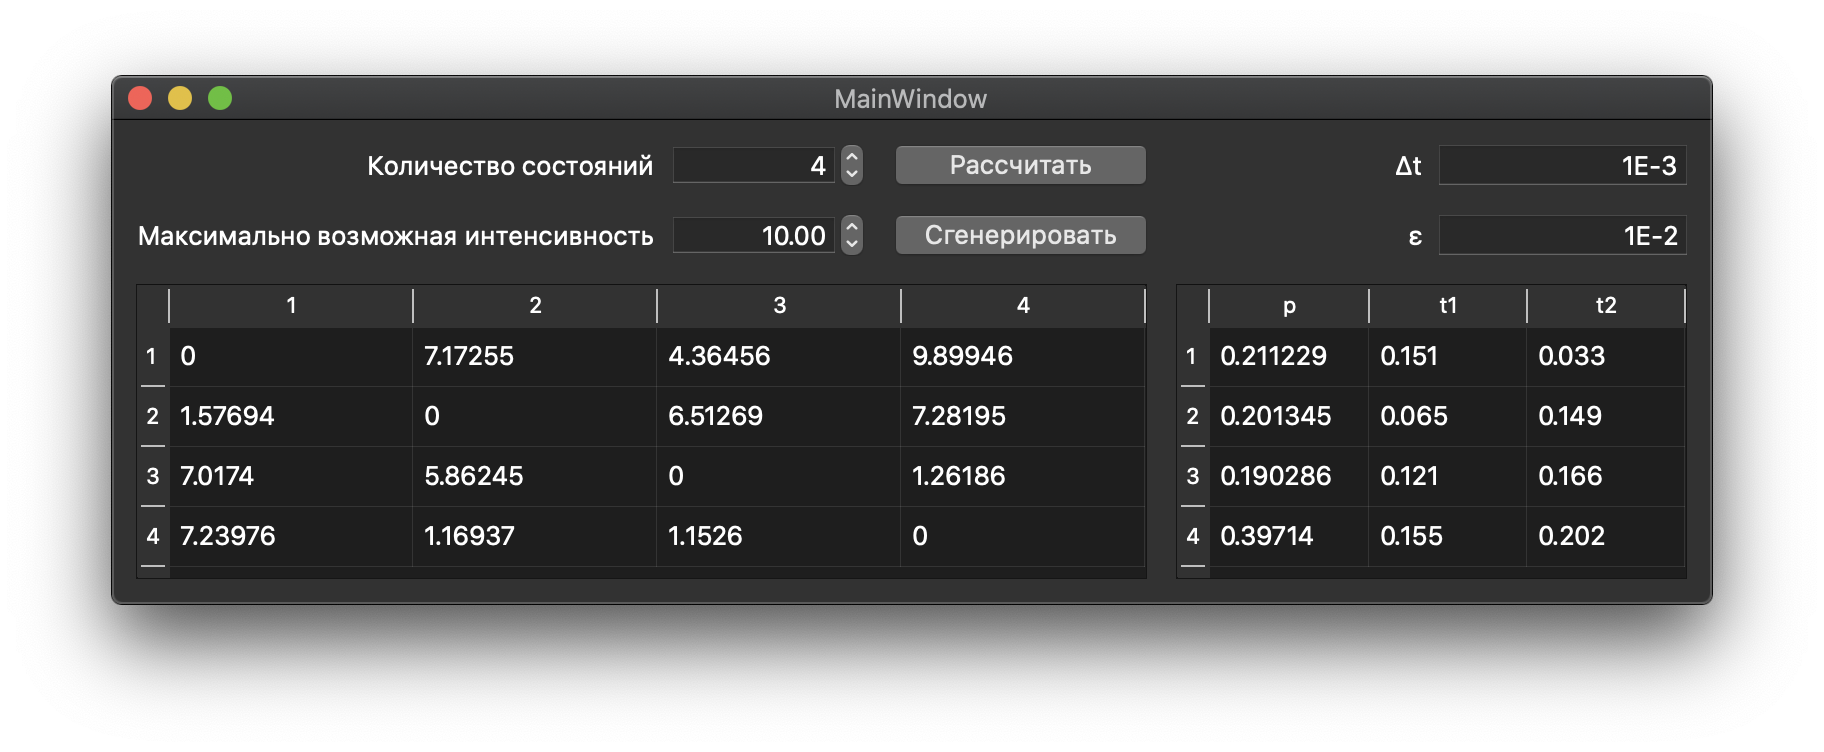
\includegraphics[width=\linewidth]{inc/img/result-4-10.png}
	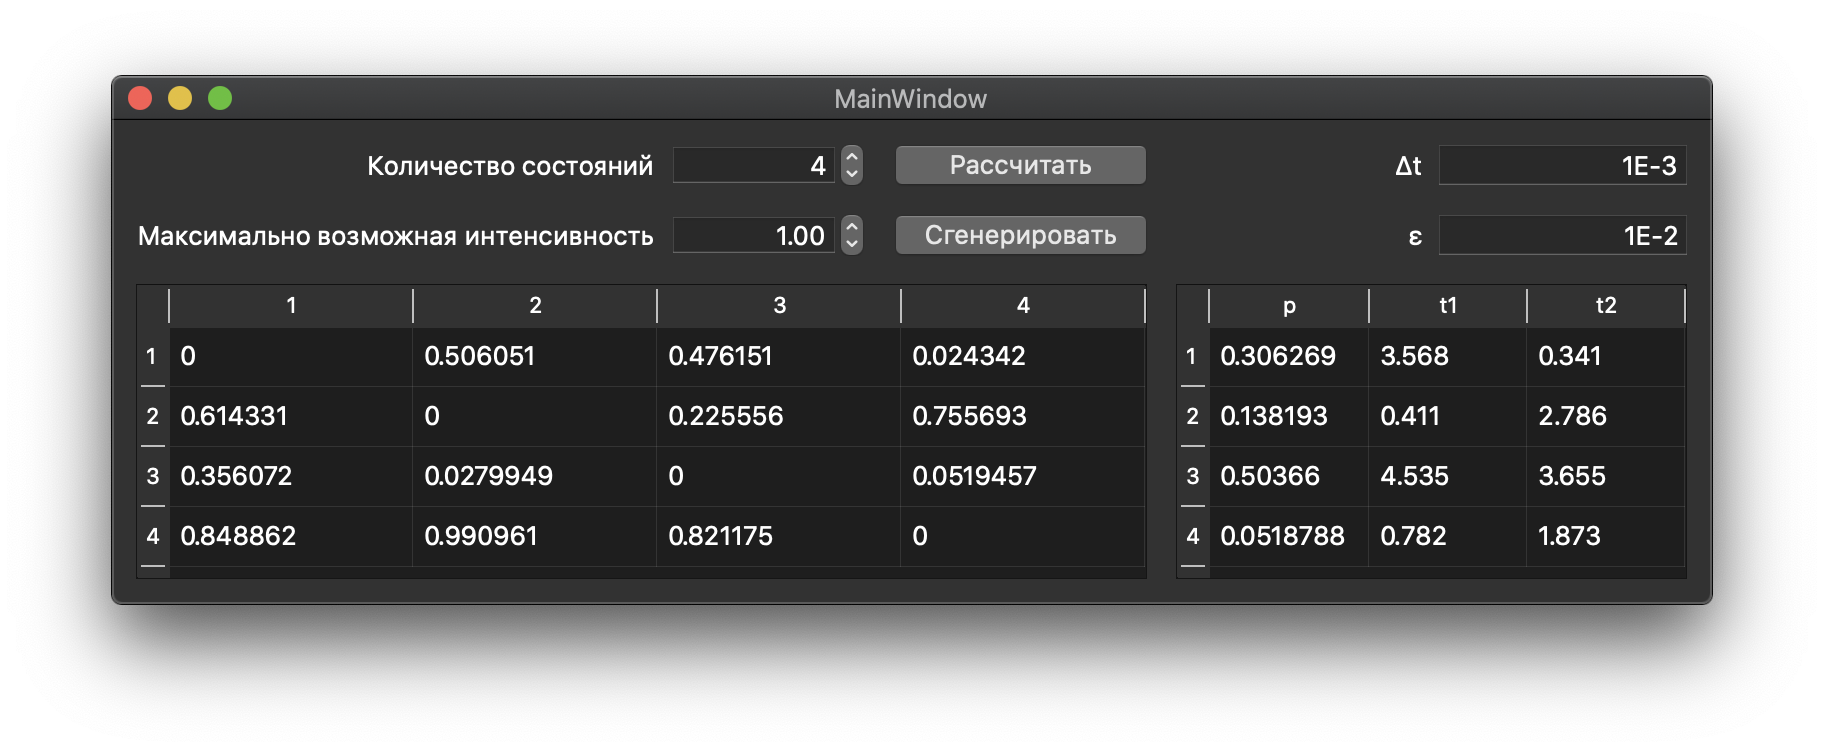
\includegraphics[width=\linewidth]{inc/img/result-4-1.png}
	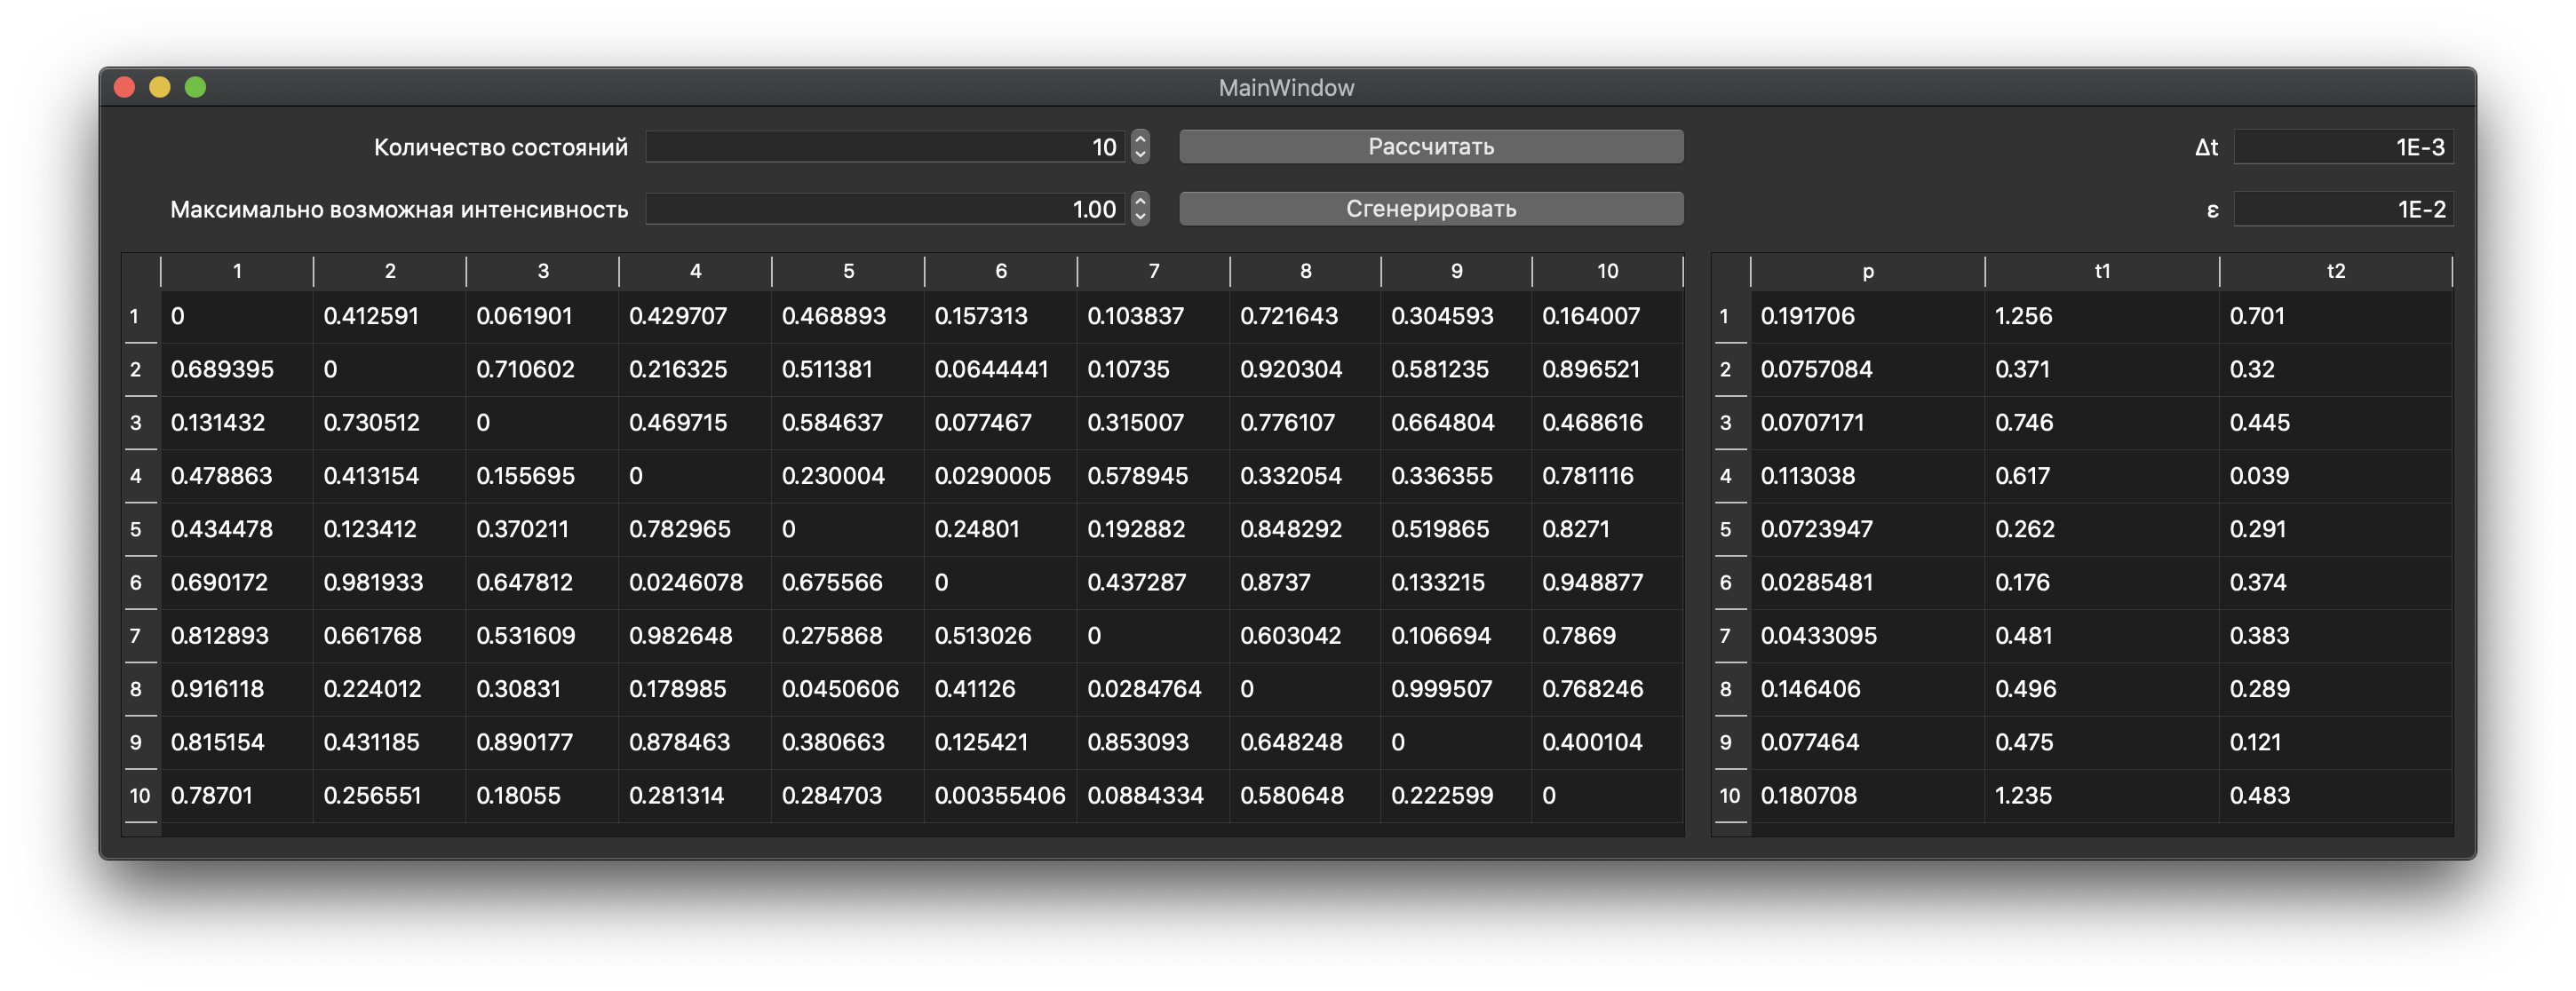
\includegraphics[width=0.95\linewidth]{inc/img/result-10-1.png}
	\caption{Результаты работы программы}
	\label{img:result}
\end{figure}

\chapter*{Вывод}
\addcontentsline{toc}{chapter}{Вывод}

Рассмотрены и смоделированы марковский процессы.
По результатам работы программы видно, что времена стабилизаций состояний значительно разятся в зависимости от вероятностей состояний системы в начальный момент времени.

Можно также заметить, что времена стабилизаций состояний уменьшаются
\begin{itemize}
	\item с увеличением количества состояний;
	\item с увеличением значений интенсивностей переходов.
\end{itemize}

\end{document}
